%----------
%---INTRODUÇÃO

\chapter{INTRODUÇÃO}
\thispagestyle{myheadings}

Este template em \LaTeX\ foi desenvolvido pelo \textbf{Prof. Dr. José Wilker de Lima Silva} (UEPB) com o objetivo de facilitar a elaboração de trabalhos acadêmicos em conformidade com as normas da ABNT. Além de fornecer uma estrutura organizada para monografias, dissertações e teses, o template reúne exemplos dos principais recursos do \LaTeX, como capítulos, seções, subseções, citações, figuras, tabelas, equações, listas, nomenclaturas, algoritmos e referências bibliográficas. Sugestões, correções e melhorias são sempre bem-vindas e contribuirão para o aperfeiçoamento contínuo deste material. \sigla{UEPB}{Universidade Estadual da Paraíba}

Este capítulo tem como objetivo apresentar exemplos de utilização dos principais recursos disponíveis neste template. Os textos, figuras, citações e demais elementos apresentados possuem caráter meramente ilustrativo e devem ser substituídos pelo conteúdo do trabalho.

Como exemplo de \textit{citação indireta}, utiliza-se o comando `\verb|\cite{}|`, conforme ilustrado a seguir: a presente pesquisa tem como objetivo principal apontar as adequações e as impropriedades frequentemente observadas na produção escrita de gêneros acadêmicos, em especial do artigo científico, a fim de traçar caminhos para o desenvolvimento de um texto de qualidade \cite[p. 200]{de2018proposito}.

Quando o nome do autor faz parte da redação da frase, recomenda-se utilizar o comando `\verb|\citeonline{}|`, como no exemplo a seguir: \citeonline{de2018proposito} verificam a necessidade de harmonia entre os elementos linguísticos e extralinguísticos na produção dos gêneros acadêmicos.

\begin{figure*}[ht!]
    \centering
    \caption{Entrada do Campus I da UEPB.}\label{fig:malha}
    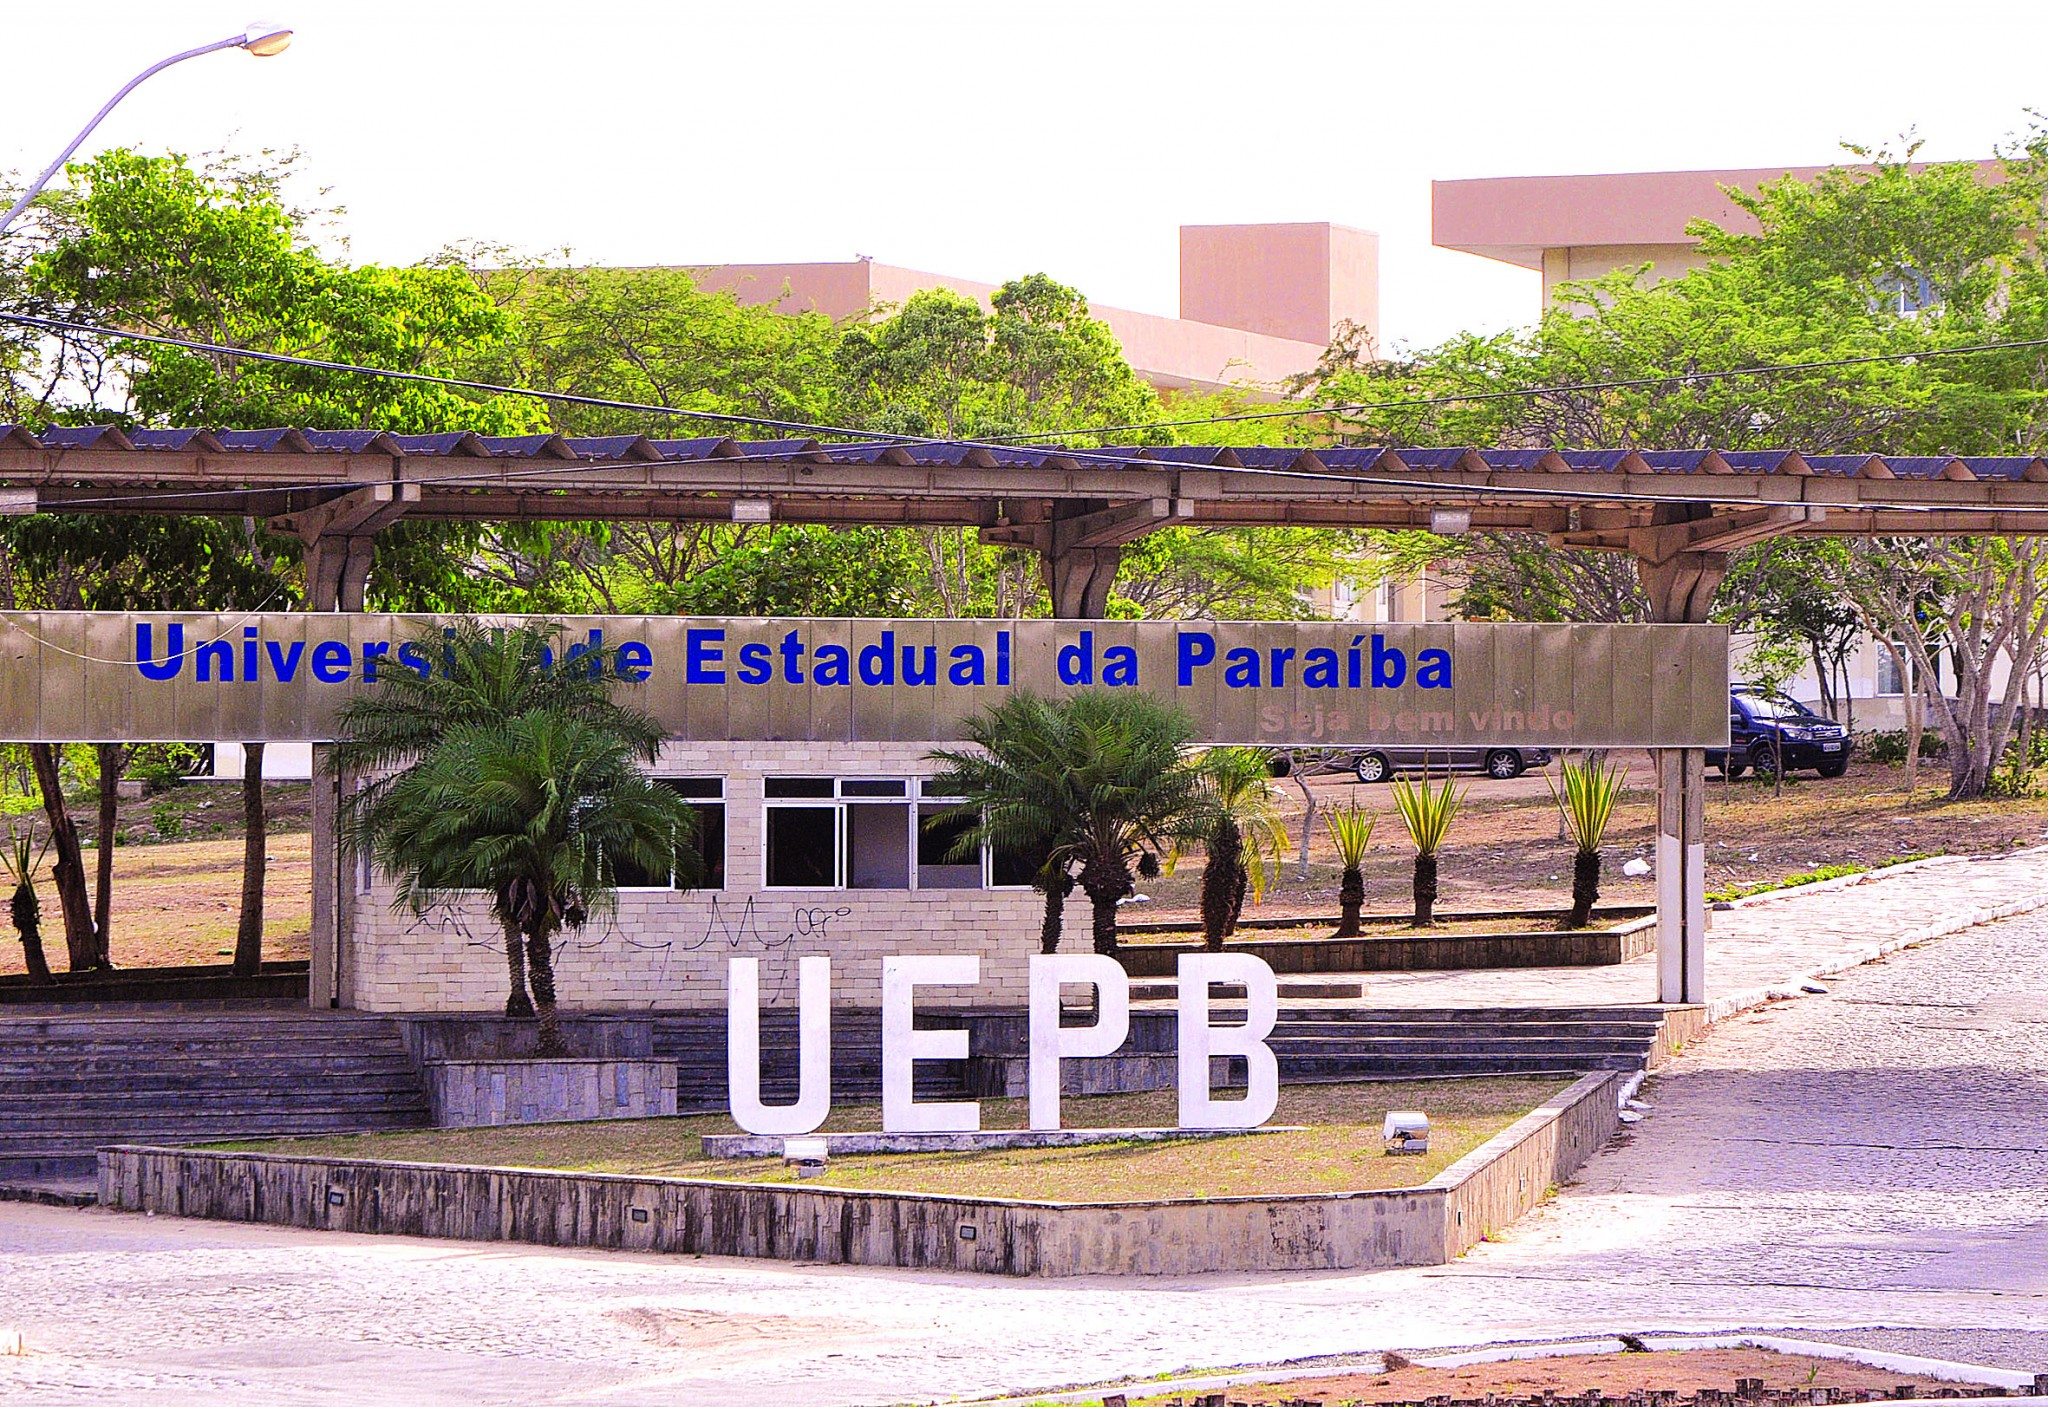
\includegraphics[width=0.8\textwidth]{imagens/entrada-uepb}\\
    {\small Fonte: Autoria própria.}
\end{figure*}

A Figura~\ref{fig:malha} exemplifica a inserção de figuras por meio do ambiente `figure`, incluindo legenda, rótulo (`label`) e referência cruzada no texto utilizando o comando `\verb|\ref{}|`. O comando

\begin{verbatim}
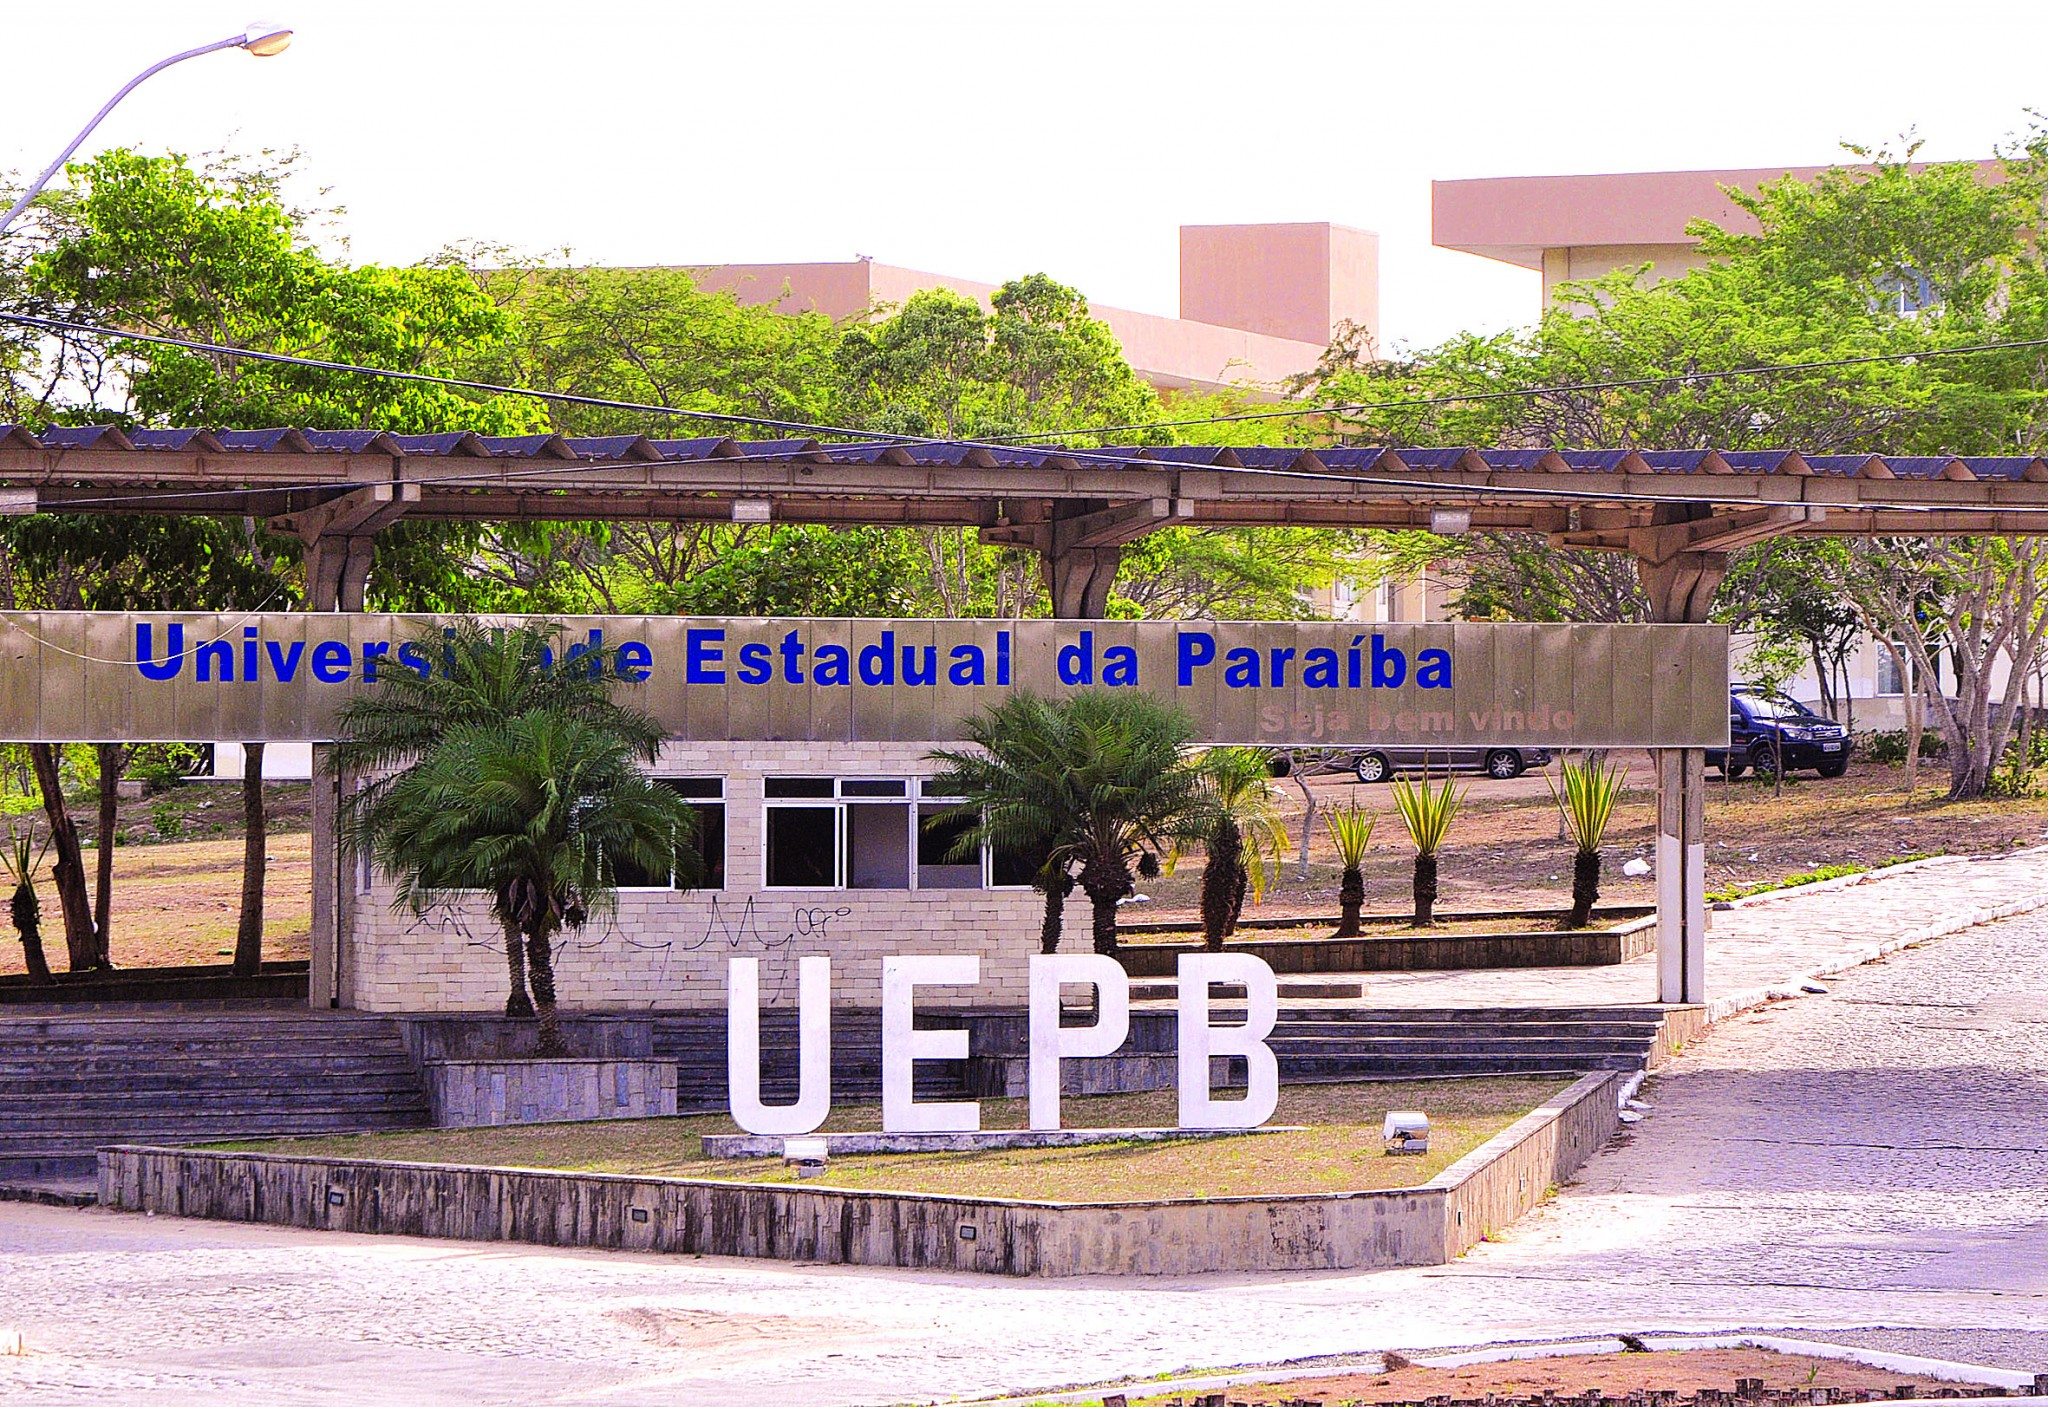
\includegraphics[width=0.8\textwidth]{imagens/entrada-uepb.jpg}
\end{verbatim}

insere a imagem \texttt{entrada-uepb.jpg} localizada na pasta \texttt{imagens}. O argumento opcional

\begin{verbatim}
[width=0.8\textwidth]
\end{verbatim}

controla o tamanho da figura, onde:

\begin{itemize}
    \item \verb|width| especifica que será definida a \textbf{largura} da imagem;
    \item \verb|0.8| indica que a figura ocupará \textbf{80\%} da largura disponível para o texto;
    \item \verb|\textwidth| representa a largura da área útil do texto da página, excluindo as margens.
\end{itemize}

Dessa forma, a imagem é redimensionada automaticamente, preservando sua proporção original.

Alguns exemplos de utilização são apresentados a seguir:

\begin{verbatim}
\includegraphics[width=0.5\textwidth]{figura}
\end{verbatim}

A figura ocupará 50\% da largura do texto.

\begin{verbatim}
\includegraphics[width=\textwidth]{figura}
\end{verbatim}

A figura ocupará toda a largura disponível do texto.

\begin{verbatim}
\includegraphics[width=6cm]{figura}
\end{verbatim}

A figura terá largura fixa de 6 cm.

Também é possível definir a altura da imagem utilizando o parâmetro \verb|height| ou combinar diferentes opções de redimensionamento conforme a necessidade do documento.

O exemplo seguinte ilustra a formatação de uma \textbf{citação direta longa}, conforme recomendado pela ABNT, utilizando recuo de 4 cm, fonte 10 pt e espaçamento simples.

\begin{adjustwidth}{4cm}{0cm} 
\small \singlespacing 
Este é apenas um texto ilustrativo para demonstrar a formatação de uma citação direta longa. Substitua-o pelo trecho original a ser citado, incluindo a referência bibliográfica correspondente e, quando aplicável, a indicação da página.
\end{adjustwidth}

Os demais capítulos deste template apresentam exemplos semelhantes para tabelas, equações, algoritmos, listas, referências bibliográficas e demais elementos frequentemente utilizados na elaboração de trabalhos acadêmicos em conformidade com as normas da ABNT.

Ao redigir o seu trabalho acadêmico, é fundamental manter o padrão na apresentação de termos técnicos. Por exemplo, ao introduzir a \sigla{UEPB}{Universidade Estadual da Paraíba} no texto pela primeira vez, o comando se encarregará de imprimir aqui no parágrafo e também na página LISTA DE ABREVIATURAS E SIGLAS o termo completo seguido da sigla entre parênteses. O mesmo comportamento automático ocorrerá ao mencionarmos a \sigla{UFPB}{Universidade Federal da Paraíba} ou a \sigla{ABNT}{Associação Brasileira de Normas Técnicas}. Para utilizar essa funcionalidade no decorrer dos seus parágrafos, você não precisa digitar tudo manualmente; basta utilizar o comando diretamente no código-fonte, escrevendo \verb|\sigla{SIGLA}{Significado Completo da Sigla}|. Outros exemplos:

\begin{verbatim}
\sigla{UEPB}{Universidade Estadual da Paraíba}
\sigla{UFPB}{Universidade Federal da Paraíba}
\sigla{UFCG}{Universidade Federal de Campina Grande}
\sigla{IFPB}{Instituto Federal da Paraíba}
\sigla{USP}{Universidade de São Paulo}
\sigla{UNICAMP}{Universidade Estadual de Campinas}
\sigla{UFRJ}{Universidade Federal do Rio de Janeiro}
\sigla{UFMG}{Universidade Federal de Minas Gerais}
\end{verbatim}
